\section{Introduction} \label{sec:intro}

\subsection{Background} \label{sec:background}
With a increasingly higher number for devices connected to the internet \cite{iot_stats}, more devices than ever are vulnerable. Many house owners do not want a wireless lock in their house, since there is a chance it can be hacked. The lock must of course be secure and resistant to attacks. However, it is hard to create something that is a hundred percent secure. This challenge is even more important for industrial systems, where loss of money, damage to the environment or even loss of lives may be consequences of system failure. There are already many examples of cyber-attacks on industrial systems, for example STRUXNET\cite{struxnet}, a computer worm that infected an Iranian nuclear facility. 
As with other industries, the marine and offshore industries are connecting more parts of their Cyber-Physical Systems(CPS) to the internet to improve their efficiency. While a number of the Cyber-Physical Systems connected to the internet are well maintained and secure, many others are vulnerable. This is most often because the CPSs are not set up properly or they run outdated software. Apart from this, it is a "fact" of statistics that if a quantity of Cyber-Physical Systems are connected to the internet, a share of these will be insecure. 

The IT security standard for industrial communication networks, IEC62443 describes preliminary recommendations and guidance for the use of cybersecurity technology and countermeasures. To stay as secure as possible, the industries should apply these measures.\cite{IEC62443} Among other things, it specifies that firewalls should be added to systems that have the ability to "[Filter] IP-addresses on the outside allowed on the inside and vice versa". And filter "[ports and] applications allowed for communication". In other words, devices should be connected to the internet only if there are good reasons for doing so.

DNV-GL is an independent expert in risk management and quality assurance, and a big share of their focus is on the maritime and offshore businesses. The DNV-GL has a Cyber Security team that helps customers assess and manage risks related to cyber security,~\cite{DNVGL_cybersec} and may therefore be interested in the findings of this project.

The research within cybersecurity at NTNU is mostly done at the Department of Information Security and Communication Technology and  the Department of Computer Science. As cybersecurity is important, other departments should put extra focus on the topic, where it is relevant.
This is the case for the Department of Engineering Cybernetics, which have a lot of focus on computer systems, both for the industry and embedded systems. Project theses like this one can be a way for the departments to get more insight in the importance of cybersecurity.

\subsection{Objectives} \label{sec:objectives}
The goal of this project is to map Cyber-Physical Systems(CPS) in the maritime and offshore industries reachable through the internet, and by doing so, get an overview of the exposure of these cyber-physical systems.

This goal was split into tasks, which define that this project should
\begin{enumerate}
    \item Introduce and define some key terms and concepts related to cybersecurity.
    \item Explain what is meant by a cyber-physical system and why cybersecurity is a topic of concern for such systems.
    \item Identify and explain search tools that can be used to identify public cyber-physical systems, focusing on the equipment and systems used in the maritime and offshore oil and gas industries. 
    \item Prepare a specification for how a search can be carried out with one or more of the identified tools. Explain the rationales for the choices made in relation to the search, for example for delimiting the outcomes.
    \item Document the results of applying the tools and elaborate on the findings.
    \item Identify potential topics that may require further research, based on the findings and in collaboration with the supervisors.
\end{enumerate}


Open-source intelligence(OSINT) is utilized to map the CPS. The OSINT search engine \href{https://shodan.io}{\color{blue}{Shodan}}\cite{shodan} is a popular search engine for enumerating Internet-connected systems, and will be used as the main reconnaissance tool of this project. 
Since most publicly available devices are already scanned and indexed by Shodan, the challenge will be to recognize devices of CPS limited to the maritime and offshore industries.


\subsection{Limitations and assumptions} \label{sec:limits}
Based on the findings at the time when this report is written, it is assumed in \cref{sec:ipv6} that the offshore and maritime industries will not use a significant amount of IPv6. Due to this, IPv6 was not investigated as thoroughly as IPv4.

Shodan is used as the main OSINT tool in this report. Any shortcomings of this tool will also affect the work of this project.

There are other tools available as well. Some of them have the same functionality as Shodan, like \href{https://censys.io/}{\color{blue}{Censys}}\cite{censys} and \href{www.zoomeye.org}{\color{blue}{ZoomEye}}\cite{zoomeye}. Other tools, like the Traceroute tool used in \cref{sec:latency_method}, cover functionalities that Shodan does not cover. There are many OSINT tools available, and while Shodan was assessed to be the most fitting for this project, parts of it might have been easier or more efficient if other tools had been used. Tools not mentioned in this report were either not found or considered as not relevant.

Honeypot technology is to make a computer pretend to be another device. This is done in order to log attempts to access the impersonated systems. This technology is quite popular for use on CPSs, and during the research of this project, multiple other articles were found that set up honeypots as part of their research.\cite{bodenheim_butts_dunlap_mullins_2014}\cite{ICS_shodan_article} Because of this, there is a chance that some of the devices found by Shodan are in reality fake. Shodan has a function for identifying honeypots, but it is not foolproof.

A device connected to the internet may have multiple different IP addresses associated with it. In this project, it is assumed that every IP address is a single device, as this is usually the case.


\subsection{Research approach} \label{sec:research_approach}
The work of this project will mostly be intelligence: To suggest methods for detecting devices as per the project goal. In this report, all mentions of "method" will refer to these methods.
To achieve the project goal in an efficient way, an certain approach is followed.
The first step will be to become familiar with the Open-source Intelligence tools useful for the purpose of identifying and analyzing devices connected to the internet. 

Research will be made in order to see what methods already exist. These methods will be tested to find out if they can be used for the purpose of this project. Then the supervisors from DNV-GL and NTNU will be consulted for thoughts on the methods found. Changes will be made to the methods according to the feedback. Iterations of the methods will then be evaluated. Based on the new results, individual research is again performed, thus completing the loop illustrated in \cref{fig:workflow} This process will be repeated until the interested parties are satisfied. 

%The main focus of this research approach is to identify and suggest use of existing methods.
The research mentioned in this approach was mainly done by finding and reading articles on the subject. These articles were found by using the search engines Engineering Village\cite{engineering_village} and Google Scholar\cite{google_scholar}. During the research, however, some OSINT techniques were easier to find in online blogs. These were found by utilizing the DuckDuckGo internet search engine\cite{ddg}. 


\tikzset{every picture/.style={line width=0.75pt}}
 
\begin{tabular}{p{10cm}}

    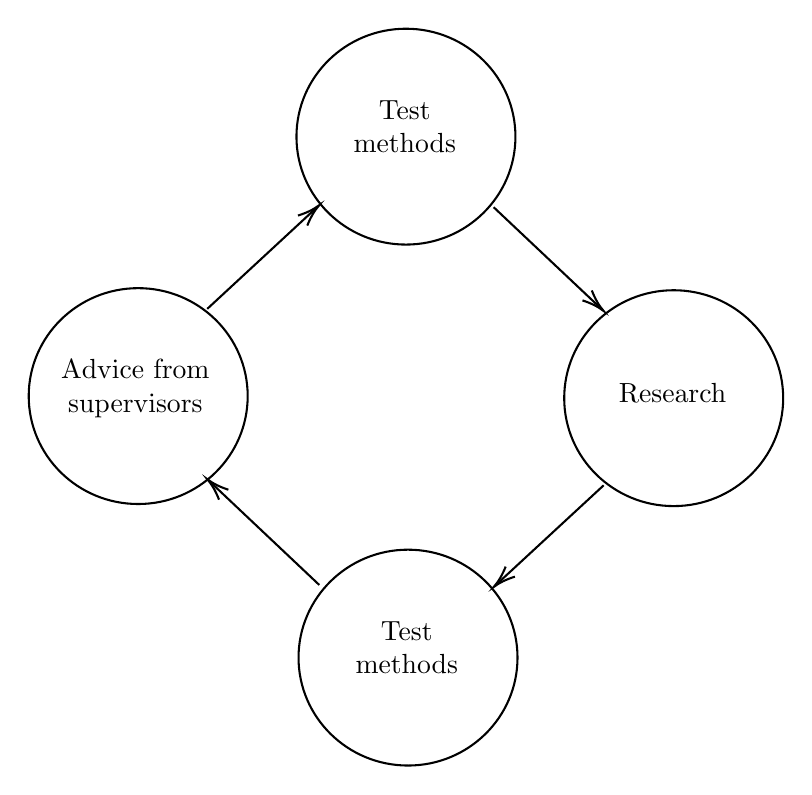
\begin{tikzpicture}[x=0.75pt,y=0.75pt,yscale=-1,xscale=1]
        %uncomment if require: \path (0,427); %set diagram left start at 0, and has height of 427

        %Shape: Ellipse [id:dp8381675984532289] 
        \draw   (107.5,211) .. controls (107.5,182.28) and (131.12,159) .. (160.25,159) .. controls (189.38,159) and (213,182.28) .. (213,211) .. controls (213,239.72) and (189.38,263) .. (160.25,263) .. controls (131.12,263) and (107.5,239.72) .. (107.5,211) -- cycle ;
        %Shape: Ellipse [id:dp8879090651544747] 
        \draw   (236.5,86) .. controls (236.5,57.28) and (260.12,34) .. (289.25,34) .. controls (318.38,34) and (342,57.28) .. (342,86) .. controls (342,114.72) and (318.38,138) .. (289.25,138) .. controls (260.12,138) and (236.5,114.72) .. (236.5,86) -- cycle ;
        %Shape: Ellipse [id:dp159469530573498] 
        \draw   (365.5,212) .. controls (365.5,183.28) and (389.12,160) .. (418.25,160) .. controls (447.38,160) and (471,183.28) .. (471,212) .. controls (471,240.72) and (447.38,264) .. (418.25,264) .. controls (389.12,264) and (365.5,240.72) .. (365.5,212) -- cycle ;
        %Shape: Ellipse [id:dp6243045365348194] 
        \draw   (237.5,337) .. controls (237.5,308.28) and (261.12,285) .. (290.25,285) .. controls (319.38,285) and (343,308.28) .. (343,337) .. controls (343,365.72) and (319.38,389) .. (290.25,389) .. controls (261.12,389) and (237.5,365.72) .. (237.5,337) -- cycle ;
        %Straight Lines [id:da3764417411513329] 
        \draw    (193.5,169) -- (246.03,120.36) ;
        \draw [shift={(247.5,119)}, rotate = 497.2] [color={rgb, 255:red, 0; green, 0; blue, 0 }  ][line width=0.75]    (10.93,-3.29) .. controls (6.95,-1.4) and (3.31,-0.3) .. (0,0) .. controls (3.31,0.3) and (6.95,1.4) .. (10.93,3.29)   ;
        %Straight Lines [id:da08718773032378624] 
        \draw    (384.5,254) -- (332.97,301.64) ;
        \draw [shift={(331.5,303)}, rotate = 317.25] [color={rgb, 255:red, 0; green, 0; blue, 0 }  ][line width=0.75]    (10.93,-3.29) .. controls (6.95,-1.4) and (3.31,-0.3) .. (0,0) .. controls (3.31,0.3) and (6.95,1.4) .. (10.93,3.29)   ;
        %Straight Lines [id:da9455012657988889] 
        \draw    (331.5,120) -- (383.05,168.63) ;
        \draw [shift={(384.5,170)}, rotate = 223.32999999999998] [color={rgb, 255:red, 0; green, 0; blue, 0 }  ][line width=0.75]    (10.93,-3.29) .. controls (6.95,-1.4) and (3.31,-0.3) .. (0,0) .. controls (3.31,0.3) and (6.95,1.4) .. (10.93,3.29)   ;
        %Straight Lines [id:da04085276077852196] 
        \draw    (247.5,302) -- (194.95,252.37) ;
        \draw [shift={(193.5,251)}, rotate = 403.36] [color={rgb, 255:red, 0; green, 0; blue, 0 }  ][line width=0.75]    (10.93,-3.29) .. controls (6.95,-1.4) and (3.31,-0.3) .. (0,0) .. controls (3.31,0.3) and (6.95,1.4) .. (10.93,3.29)   ;

        % Text Node
        \draw (259.25,67) node [anchor=north west][inner sep=0.75pt]   [align=left] {\begin{minipage}[lt]{41.865356pt}\setlength\topsep{0pt}
            \begin{center}
                Test \\methods
            \end{center}

        \end{minipage}};
        % Text Node
        \draw (117.75,192) node [anchor=north west][inner sep=0.75pt]   [align=left] {\begin{minipage}[lt]{59.42064400000001pt}\setlength\topsep{0pt}
            \begin{center}
                Advice from \\supervisors
            \end{center}

        \end{minipage}};
        % Text Node
        \draw (385.25,203.5) node [anchor=north west][inner sep=0.75pt]   [align=left] {\begin{minipage}[lt]{46.398644000000004pt}\setlength\topsep{0pt}
            \begin{center}
                Research
            \end{center}

        \end{minipage}};
        % Text Node
        \draw (260.25,318) node [anchor=north west][inner sep=0.75pt]   [align=left] {\begin{minipage}[lt]{41.865356pt}\setlength\topsep{0pt}
            \begin{center}
                Test \\methods
            \end{center}

        \end{minipage}};


    \end{tikzpicture}

    \captionof{figure}{Illustration of workflow}
    \label{fig:workflow}
\end{tabular}



\subsection{Structure of report}
This report has five main parts. First, in this section, \cref{sec:intro}, the project is introduced. In \cref{sec:theory}, basic principles used in this project are explained. 
Important principles from the working of the internet are explained, along with the basics of the Shodan search engine. In \cref{sec:method}, different methods for selective identification of IP devices are outlined. In \cref{sec:results}, the results from using the aforementioned methods are listed, along with a discussion of these results. In \cref{sec:conclusion}, a conclusion is drawn from the results.  Finally, further work on the topic is suggested in \cref{sec:further_work}.

\newpage
